% arara: lualatex
% arara: biber
% arara: lualatex
% arara: lualatex if found('log', 'undefined references')

% classe do documento ----------------------------------------------------
\documentclass[12pt]{article}

% fontes e cia
\usepackage{euler}
\usepackage{fontspec}
\usepackage{libertine}

% idioma
\usepackage[brazilian]{babel}

% margem
\usepackage[a4paper]{geometry}

% protusão 
\usepackage{microtype}

% math 
\usepackage{amsmath, amsthm, amssymb}

% figutas, tabelas, seções, etc
\usepackage{tabularray}
\usepackage{graphicx}
  \graphicspath{{./figs}}
\usepackage[font = {small, sf}, labelfont = {bf, sf}]{caption}
\usepackage{sectsty}
  \allsectionsfont{\sffamily}

% referências bibliográficas
\usepackage[style=abnt, justify]{biblatex}
  \addbibresource{bib/referencias.bib}

% metadados
\usepackage{hyperref}
  \hypersetup{%
    colorlinks  = true, 
    linkcolor   = blue, 
    urlcolor    = blue, 
    citecolor   = blue,
    pdfproducer = {LuaLaTeX},
    pdfcreator  = {LaTeX2e com neovim e arara},
    pdftitle    = {Artigo Genérico Isento de Sentido}, 
    pdfauthor   = {Fulano de Tal},
    pdfsubject  = {Estudo Dirigido para aprendizagem do LaTeX}, 
    pdfkeywords = {tex, latex, math}
  }

% numeração de ata
\usepackage{lineno}
%  \linenumbers

% configurações do título ---------------------------------------------->>
\title{%
  \sffamily \bfseries
  Artigo Genérico Isento de Sentido
}
\author{%
  \sffamily 
  Fulano de Tal \thanks{fulantal@email.com}
}
\date{%
  \sffamily
  \today
}
%-----------------------------------------------------------------------<<

% ambientes matemáticos ------------------------------------------------>>
\theoremstyle{plain}
  \newtheorem{teorema}{\sffamily Teorema}[section]
  \newtheorem{corolario}{\sffamily Corolário}[teorema]
  \newtheorem{proposicao}{\sffamily Proposição}[section]
\theoremstyle{definition}
  \newtheorem{definicao}{\sffamily Definição}[section]
  \newtheorem{exemplo}{\sffamily Exemplo}
  \newtheorem{lema}{\sffamily Lema}[section]
\theoremstyle{remark}
  \newtheorem{obs}{\sffamily Observação}
  \newtheorem*{paradoxo}{\sffamily Paradoxo de Bernouli}
%-----------------------------------------------------------------------<<

% novos operadores ----------------------------------------------------->>
\DeclareMathOperator{\sen}{sen}
\DeclareMathOperator{\arcsen}{arcsen}
%-----------------------------------------------------------------------<<


% início do documento ====================================================
\begin{document}
%-----------------------------------------------------------------------
  \maketitle
%
  %===========================================================================
% Resumo 
%===========================================================================

\begin{abstract}
  Esse é um pequeno resumo sobre o texto. 
  Seja objetivo e destaque pontos relevantes. 
  Em nosso caso, esse texto versará sobre um artigo genérico e, em muitos 
  pontos, provavelemente, isento de sentido. 
  Tem por objetivo ser usado para um momento prático de um quase microcurso sobre 
  \LaTeX\ ministrado no \textsf{II Colóquio de Matemática do CFP}. 
\end{abstract}


%
  \tableofcontents
%
  % Seção 01: O Corpo Complexo ===============================================

\section{O Corpo dos Números Complexos}
\label{sec:corpo}

Definir o Conjunto dos Números Complexos, inicialmente, por 
\[
  \mathbb{C} = \left\{\, a + bi; \; a,b \in \mathbb{R} \text{ e } i^2 = -1 \,\right\},
\]
pode esconter algumas coisas fundamentais no entendimento desse novo conjunto. 
Afinal\ldots\ 
Seria essa soma entre $a$ e $bi$ é usual?
O que significa $i^2 = -1$?
Como você explicaria o seguinte Paradoxo?

\begin{paradoxo}
  Considerando, $ i^2 = -1$, temos:
  \[
    -1 = i^2 = i \cdot i = \sqrt{-1}\cdot \sqrt{-1} = \sqrt{(-1)(-1)} = \sqrt{1} = 1
  \]
Portanto, $-1 = 1$?
\end{paradoxo}

Mas, como Gauss já dizia: \textit{Na Matemática não existem controvérsias verdadeitas}! 

Faz-se necessário uma formalização na definição dos números complexos. 

\subsection{Formalizando as coisas} %---------------------------------------

Precisamos entender os Númetos Complexos não como uma ``sacola de números'', mas 
como uma ``corpo de números'', ou seja, um conjunto com uma estrutura algébrica 
associada, preferencialmente já conhecida.

Hamilton, matemático, físico e astrónomo irlandês, foi que trouxe uma definição 
adequada aos números complexos, sendo adotada até os dias atuais. 
Nela vê-se o conjunto dos números complexos como um conjunto de pares ordenados 
munidos com as operações de soma e produdo, este último bem peculiar, mas que 
oferece subsídios para verificar que essa estrutura é um Corpo. 


\begin{proposicao}
  Considere o subconjunto $\mathcal{C} \subset \mathbb{R}^2$, não vazio, munido 
  das seguintes operações de \textsf{soma} e \textsf{produdo}, dadas por 
  \[
    \begin{array}{rcc}
      + \colon \mathcal{C}\times \mathcal{C} & \to & \mathcal{C} \\
       (x, y) & \mapsto & x + y 
    \end{array}
    \quad 
    \text{ e }
    \quad 
    \begin{array}{rcc}
      \cdot \colon \mathcal{C}\times \mathcal{C} & \to & \mathcal{C} \\
       (x, y) & \mapsto & x \cdot y 
    \end{array}
  \]
  Então, são satisfeitas as seguintes condições, para $z,w,t \in \mathbb{C}$:

  \begin{enumerate}
      \item[(i)] $z + (w + t) = (z + w) + t$
      \item[(ii)] $z + w = w + z$
      \item[(iii)] $ \exists\ 0 \in \mathcal{C}$, tal que $z + 0 = z$
      \item[(iv)] $ \exists\ -z \in \mathcal{C}$, tal que $ z + (-z) = 0 $
      \item[(v)] $z(wt) = (zw)t$
      \item[(vi)] $zw = wz$
      \item[(vii)] $ \exists\ 1 \in \mathcal{C} $, tal que $z \cdot 1 = z$, $\forall z$
      \item[(viii)] $ \exists\ z^{-1} \in \mathcal{C}$, tal que $z\cdot z^{-1} = 1$, para todo $z \neq 0$
      \item[(ix)] $ z (w + t) = zw + zt  $
  \end{enumerate}  
\end{proposicao}

\begin{definicao}[Corpo dos Números Complexos]
  A esse conjunto $\mathcal{C}$, definido acima, denominamos \textsf{Corpo dos Números Complexos} e 
  será denotado por $\mathbb{C}$.
\end{definicao}

\begin{obs}
  É possível mostrar algumas identificaçãos, tais como 
  \begin{enumerate}
    \item $ (x, 0) \sim x $
    \item $ (0, 1)^2 = -1 $
    \item $ (0, y) \sim yi $
  \end{enumerate}
  Assim, um número complexo $ z = (x, y) $, pode ser identificado por 
  \begin{align}
    z &= (x, y) \notag\\
      &= (x, 0) + (0, y) \notag \\
      &= x + yi \label{eq:algebrica}
  \end{align}
\end{obs}

Dizemos que \eqref{eq:algebrica} está na \textbf{Forma Algébrica}. 

\subsection{Representação Matricial} %--------------------------------------

Também é possível representar um número complexo $ z = a + bi $, na forma 
\textbf{Matricial}: 
\[
  z = 
  \begin{bmatrix}
    a & -b \\
    b &  a
  \end{bmatrix}
\]


  % Sec 2: TFA 

\section{Teorema Fundamental da Álgebra}
\label{sec:TFA}

Na Seção~\ref{sec:corpo}, vimos qualquer coisa sobre números complexos. 
Então, nessa seção, demonstraremos o \textsf{Teorema Fundamental da Álgebra} (TFA). 
Nunca escreva uma introdução de seção dessa forma!

Para a demonstação do \textsf{TFA} precisaríamos de todo um curso de Variáveis Complexas. 
Mas, como não é possível isso, considere que $\mathbb{C}[z]$ seja o conjunto dos 
polinômios complexos. 
Também vou considerear que você acreditará nos lemas seguintes:

\begin{lema}\label{lema:minimo}
  Seja $ f(z) \in \mathbb{C}[z] $. 
  Então, $ \vert f(z) \vert $ atinge um valor mínimo em algum ponto $ z_0 \in \mathbb{C} $
\end{lema}

\begin{lema}\label{lema:naoMinimo}
  Suponha que $ f(z) \in \mathbb{C}[z] $, sendo $ f(z) $ não constante. 
  Se $ f(z_0) \neq 0 $, então $ \vert f(z_0) \vert $ não é o valor mínimo de 
  $ \vert f(z) \vert $. 
\end{lema}

\begin{teorema}[Teorema Fundamental da Álgebra]
  Se $ f(z) \in \mathbb{C}[z] $, com $ f(z) $ não constante; então $ f(z) $ 
  possui, pelo menos, uma raíz complexa.
\end{teorema}

\begin{proof}[Demonstração.]
  Considere $ f(z) $ um polinômio complexo não constante. 
  Pelo Lema~\ref{lema:minimo}, $ \vert f(z) \vert $ atinge um valor mínimo em 
  algum ponto $ z_0 \in \mathbb{C} $. 
  Então, pelo Lema~\ref{lema:naoMinimo}, segue-se que $ f(z_0) = 0 $; pois, 
  caso contrário, não seria o valor mínimo. 
  Portanto, $ f(z) $ possui uma raíz complexa. 
\end{proof}

Quantos anos você possui?
O que tens feito da vida até aqui? 
Pois saiba que Gauss demonstrou esse teorema\footnote{
  não foi a demonstração acima, mas uma outra com as ferramentas disponíveis à época
} aos 18 anos de idade, em sua tese de doutorado! 

\begin{figure}[!htbp]
  \centering
  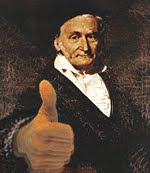
\includegraphics[width=0.3\linewidth]{leGauss}
  \caption{Gauss dando Legal}
  \label{fig:leGauss}
\end{figure}

Para mais detalhes, veja \textcite{TFA}

  % Sec 3: Cálculo Fracionário

\section{Cálculo Fracionário} % (fold)
\label{sec:fracionario}

\subsection{Derivada Fracionária} %-----------------------------------------

Você sabe que se $ f \colon X \to \mathbb{R} $ e $ a \in X \cap X^{\prime} $, 
a \textbf{derivada} da função $f$ no ponto $a$ é o limite:

\[
  f^{\prime}(a) = \lim_{h \to 0} \frac{f(a + h) - f(a)}{h}
\]

Usamos a notação $f^{n}(a)$ para a $n$-ésima derivada da função $f$. 
Quando existe $f^{n}(x)$ para todo $x\in I$, sendo $I$ um intervalo, dizemos que 
a função $f\colon I \to \mathbb{R}$ é \textit{n-vezes derivável no intervalo} $I$. 

A Tabela~\ref{tab:derivadas} lembra-nos de algumas derivadas notáveis

\begin{table}[!htbp]
  \centering
  \caption{Tabela de Derivadas}
  \label{tab:derivadas}
  \begin{tblr}{cc}
    \hline[1.6pt]
      $ f(x) $       &   $ f^\prime(x) $ \\
    \hline[0.8pt]    
      $ e^x $        &   $ e^x $ \\
      $ a^x $        &   $ a^x \ln{(a)} $ \\
      $ \arcsen{x} $ &   $ \frac{ 1 }{ \sqrt{1 - x^2} }\,\mathrm{d}x $ \\
    \hline[1.6pt]    
  \end{tblr}
\end{table}

O \textsf{\textbf{Cálculo Fracionário}} é uma área da Matemática que foi idealizada 
quando tentou-se generalizar a ideia da derivada para uma ordem \textit{arbitrária}, 
não apenas inteira. 

Você já imaginou uma derivada como $f^{1/2}(x)$? 
Ou, mais surpreendente: $f^{\sqrt{\pi}}(x)$??
Ou, absurda e mais surpreendente: $f^{2 + 3i}(z)$???

Pois é \ldots\ muitas definições surgiram ao longo da história, mas vou exibir 
uma formulação de Riemann-Liouville. 

\begin{definicao}[Derivada de Riemann-Liouville em intervalo finito]
  Uma das derivadas, em um intervalo fnito, de Riemann-Liouville, 
  $ D_{a^{+}}^{\alpha} f $, de ordem $ \alpha \in \mathbb{C} $ com 
  $\textrm{Re}(\alpha) \geq 0$ e $ \alpha \not \in \mathbb{N}$, é definida por:
  \begin{equation}
    \left(D_{a^{+}}^{\alpha}f\right)(x) = 
    \frac{1}{\Gamma(n - \alpha)}
    \left(
      \frac{\mathrm{d}}{\mathrm{d}x}
    \right)^{n} 
    \int_{a}^{x} 
    \frac
    { 
      f(t)\, \mathrm{d}t
    }
    {
      (x - t)^{\alpha - n + 1}
    }
  \end{equation}
com $ n = \left[\textrm{Re}(\alpha)\right] + 1 $ e $ x > a $, sendo 
$ \left[\textrm{Re}(\alpha)\right] $ é a parte inteira de \textrm{Re}(\alpha) e 
\[
  \Gamma(z) = \int_{0}^{\infty} t^{z - 1} e^{-t}\, \mathrm{d}t,
\]
com $\textrm{Re}(z) > 0$.
\end{definicao}

Sei que é complicado!
Mas, pior, é uma análise morfossintática, não?  

\subsection{Funções de Mittag-Leffler}

Uma função, denotada por $E_{\alpha}(z)$, possui papel relevante nos estudos 
do Cálculo Fracionário. 
Isto porque, podemos interpretá-la como uma generalização da função exponencial. 

\begin{definicao}[Função de Mittag-Leffler]
  A função de Mittag-Leffler, $E_{\alpha}(z)$, é uma função complexa que depende 
  de um parâmetro complexo $\alpha$, sendo $ \textrm{Re}(z) > 0 $, é dada pela 
  série de potências:
  \[
    E_{\alpha}(z) = \sum_{k = 0}^{\infty} \frac{z^k}{\Gamma(\alpha k + 1)}
  \]
\end{definicao}

Note que, se você demonstrar a igualdade $\Gamma(k + 1) = k!$, você perceberá 
a ideia da generalização da exponencial; pois, para $ \alpha = 1 $, temos:

\begin{align*}
  E_{1}(z) &= \sum_{k = 0}^{\infty} \frac{z^k}{\Gamma(k + 1)} \\
           &= \sum_{k = 0}^{\infty} \frac{z^k}{k!} \\
           &= e^{z}
\end{align*}

Se deseja conhecer mais sobre o Cálculo Fracionário, veja \textcite{fracionario}.

%
  \nocite{*}
  \printbibliography
%
%-----------------------------------------------------------------------
\end{document}
%=========================================================================
